% Heterogeneous Edge-AI Runtime -- progress report deck.
% Build: latexmk -xelatex main.tex   (see README.md)
% Content source: docs/SLIDES_OVERVIEW.md, docs/SYSTEM_GUIDE.md, docs/research/.
% Number policy: every number is a DESIGN value, a CALCULATED value, a HOST-TEST
% result, or a PUBLISHED figure from another setup. Nothing here is a Pi/STM32 measurement.
\documentclass[aspectratio=169,12pt,t]{beamer}

% Speaker notes: uncomment ONE line to see them.
% \setbeameroption{show notes on second screen=right}  % dual-screen (pdfpc)
% \setbeameroption{show only notes}                     % notes handout

\usetheme[progressbar=none, sectionpage=none]{moloch}
% A 208 x 117 mm canvas retains 16:9 and the actual 12pt class fonts.
% Long owner-approved sentences fit without frame scaling or reduced fonts.
\geometry{paperwidth=208mm,paperheight=117mm}

% ---------- fonts ----------
\usepackage{fontspec}
\setsansfont{Avenir Next}[BoldFont={Avenir Next Demi Bold}]
\setmonofont{Menlo}[Scale=1.0]
\newfontfamily\captionface{Avenir Next Condensed}
\newcommand{\captiontype}{\captionface\fontsize{10}{11}\selectfont}

% ---------- palette ----------
\definecolor{navy}{HTML}{1F3A5F}
\definecolor{teal}{HTML}{2A9D8F}
\definecolor{fault}{HTML}{E76F51}
\definecolor{paper}{HTML}{FAFAF7}
\definecolor{ink}{HTML}{22262B}
\definecolor{muted}{HTML}{6B7280}
\definecolor{rule}{HTML}{D6D9DE}

\setbeamercolor{normal text}{fg=ink, bg=paper}
\setbeamercolor{frametitle}{fg=paper, bg=navy}
\setbeamercolor{progress bar}{fg=teal, bg=rule}
\setbeamercolor{alerted text}{fg=fault}
\setbeamercolor{example text}{fg=teal}
\setbeamercolor{structure}{fg=navy}
\setbeamercolor{title separator}{fg=teal}
\setbeamercolor{footline}{fg=muted}
% Beamer otherwise inherits the fault/alert color for in-slide citations.
\setbeamercolor{bibliography entry author}{fg=navy}
\setbeamercolor{bibliography entry title}{fg=ink}
\setbeamercolor{bibliography entry location}{fg=muted}
\setbeamercolor{bibliography entry note}{fg=muted}
\setbeamercolor{block title}{fg=paper, bg=navy}
\setbeamercolor{block body}{bg=navy!6}
\setbeamerfont{frametitle}{size=\large, series=\bfseries}
\setbeamertemplate{frametitle}{\nointerlineskip\begin{beamercolorbox}[wd=\paperwidth,sep=2mm,leftskip=4mm]{frametitle}\usebeamerfont{frametitle}\insertframetitle\strut\end{beamercolorbox}}
\setbeamertemplate{itemize items}{\color{teal}\rule[0.25ex]{0.45em}{0.45em}}
\setbeamertemplate{bibliography item}[text]
\setbeamertemplate{page number in head/foot}[totalframenumber]
\hypersetup{colorlinks=true, linkcolor=navy, urlcolor=navy, citecolor=navy}
% Keep the appendix bookmark free of Beamer translation commands.
\pdfstringdefDisableCommands{\def\translate#1{#1}}

\setbeamertemplate{itemize subitem}{\color{muted}--}

% ---------- packages ----------
\usepackage{tikz}
\usetikzlibrary{arrows.meta, positioning, automata, calc, shapes.geometric, fit, backgrounds, decorations.pathreplacing}
\usepackage{booktabs}
\usepackage{array}
\newcolumntype{L}[1]{>{\raggedright\arraybackslash}p{#1}}
\usepackage{amsmath}
\usepackage{siunitx}
\sisetup{detect-all}

% ---------- helpers ----------
\newcommand{\muted}[1]{{\color{muted}#1}}

% \slideimg[<max height>]{<width>}{<V-id>}{<caption for placeholder>}
% Shows images/<V-id>.jpg or .png if present, otherwise a labelled gray box of the same size.
\newcommand{\slideimg}[4][0.62\textheight]{%
  \IfFileExists{images/#3.jpg}{%
    \includegraphics[width=#2, height=#1, keepaspectratio]{images/#3.jpg}%
  }{\IfFileExists{images/#3.png}{%
    \includegraphics[width=#2, height=#1, keepaspectratio]{images/#3.png}%
  }{%
    \begin{tikzpicture}
      \node[draw=rule, fill=black!6, rounded corners=2pt, minimum width=\dimexpr#2-1pt\relax, outer sep=0pt,
            minimum height=#1, align=center, text width=\dimexpr#2-8mm\relax, font=\small, text=muted]
        {\textbf{#3}\\[2pt]#4\\[2pt]\small ảnh chờ bổ sung};
    \end{tikzpicture}%
  }}%
}

\tikzset{
  box/.style={draw=navy, fill=white, rounded corners=2pt, align=center, font=\small,
              minimum height=7mm, inner sep=3pt},
  flow/.style={-{Stealth[length=2mm]}, thick, color=navy},
  faultflow/.style={-{Stealth[length=2mm]}, thick, color=fault},
  lbl/.style={font=\small, color=ink, fill=paper, inner sep=1pt},
}

% Only the page number appears in the footer.
\setbeamerfont{footline}{size=\small}
\setbeamertemplate{footline}{\hbox{\begin{beamercolorbox}[wd=\paperwidth,ht=4mm,dp=1mm,rightskip=6mm]{footline}\hfill\insertframenumber/\inserttotalframenumber\end{beamercolorbox}}}
\AtBeginSection{\begin{frame}[c]\centering{\Huge\bfseries\color{navy}\thesection. \insertsectionhead\par}\end{frame}}
\setbeamertemplate{navigation symbols}{}
\setbeamersize{text margin left=6mm,text margin right=6mm}
\setlength{\tabcolsep}{4pt}
\renewcommand{\arraystretch}{1.02}
\title{Nền tảng thực thi Edge-AI không đồng nhất}
\subtitle{Heterogeneous Edge-AI Runtime}
\author{Nhóm 3 Stars}
\institute{Giảng viên hướng dẫn: TS. Nguyễn Quang Minh}
\date{07/10/2026}


\newcounter{slidefigure}
\newcommand{\figcap}[1]{\par\vspace{1pt}{\captiontype\color{muted}\refstepcounter{slidefigure}Hình \theslidefigure: #1\par}}
\setbeamerfont{bibliography entry author}{size=\small}
\setbeamerfont{bibliography entry title}{size=\small}
\setbeamerfont{bibliography entry location}{size=\small}
\setbeamerfont{bibliography entry note}{size=\small}
\setlength{\emergencystretch}{2em}
\setbeamerfont{normal text}{size=\small}
\setbeamerfont{itemize/enumerate body}{size=\small}
\setbeamerfont{itemize/enumerate subbody}{size=\footnotesize}
\linespread{0.90}
\AtBeginDocument{\setlength{\leftmargini}{1.1em}\setlength{\leftmarginii}{1.2em}\setlength{\labelsep}{.35em}}
\newcommand{\namedcap}[2]{\par\vspace{2pt}{\captiontype\color{muted}Hình #1: #2\par}}
\begin{document}
\raggedright
\setlength{\parskip}{0pt}
\begin{frame}[c]
\relax
{\centering\LARGE\bfseries\color{navy}NỀN TẢNG THỰC THI EDGE-AI\par KHÔNG ĐỒNG NHẤT\par}
\vspace{3pt}{\centering\color{teal}Heterogeneous Edge-AI Runtime\par}
{\color{teal}\hrule height .6pt}\vspace{10pt}
\begin{columns}[T,onlytextwidth]
\begin{column}{.54\textwidth}
\textbf{Nhóm thực hiện:} 3 Stars\par\vspace{5pt}
{\small\hspace{1em}Nguyễn Quốc Khánh – 20233464 (Nhóm trưởng)\par
\hspace{1em}Nguyễn Trung Hiếu – 20233398\par
\hspace{1em}Nguyễn Quang Vinh – 20233718\par}
\vspace{10pt}GVHD: TS. Nguyễn Quang Minh\par
Mã lớp bài tập: 173876
\end{column}
\begin{column}{.44\textwidth}
\centering\slideimg[.48\textheight]{\linewidth}{V01}{}
\end{column}
\end{columns}
\note{Ảnh bìa minh họa hai miền, không phải ảnh hệ thống đã lắp.}
\end{frame}
\begin{frame}{Mục lục}
\small
\Large
1. Giới thiệu\par\vspace{9pt}
2. Cơ sở lý thuyết\par\vspace{9pt}
3. Thiết kế hệ thống\par\vspace{9pt}
4. Phương pháp đánh giá\par\vspace{9pt}
5. Tiến độ và kế hoạch\par\vspace{9pt}
6. Kết luận
\end{frame}
\section{Giới thiệu}
\begin{frame}{1.1 Động lực nghiên cứu}
\small
\begin{itemize}\setlength{\itemsep}{2pt}\setlength{\parsep}{0pt}\setlength{\parskip}{0pt}\setlength{\topsep}{0pt}
\item Trí tuệ nhân tạo (AI, Artificial Intelligence) đang được đưa xuống thiết bị biên (edge): robot, drone, xe tự hành, máy công nghiệp chạy mạng nơ-ron ngay trên máy tính nhúng chạy Linux.
\begin{itemize}\setlength{\itemsep}{2pt}\setlength{\parsep}{0pt}\setlength{\parskip}{0pt}\setlength{\topsep}{0pt}
\item Lý do: phản hồi nhanh, không phụ thuộc mạng, dữ liệu không rời thiết bị.
\end{itemize}
\item Kết quả AI không chỉ để hiển thị mà được dùng để \textbf{điều khiển} cơ cấu vật lý (động cơ, phanh, cánh tay robot).
\item Với hệ điều khiển, một kết quả \textbf{đúng nhưng đến muộn} cũng nguy hiểm như một kết quả sai.
\item Câu hỏi đặt ra: hệ điều hành chạy AI có bảo đảm được \emph{thời điểm} kết quả đến hay không?
\end{itemize}
\vspace{12pt}
Hình 1a cho thấy thời hạn nằm ở đầu ra điều khiển, không chỉ ở phép suy luận.
\par\vspace{8pt}
\begin{minipage}{\linewidth}\centering
\begin{tikzpicture}[node distance=18mm,box/.append style={minimum width=35mm,minimum height=12mm}]
\node[box] (sensor) {Cảm biến};
\node[box,right=of sensor] (ai) {AI trên Linux};
\node[box,right=of ai] (control) {Điều khiển};
\draw[flow] (sensor)--(ai);\draw[flow] (ai)--(control);
\draw[flow,teal] (control.south)--++(0,-.7)-|node[pos=.25,below,font=\small]{Hệ vật lý phản hồi qua cảm biến} (sensor.south);
\end{tikzpicture}
\namedcap{1a}{Vòng cảm biến–AI–điều khiển: dữ liệu phải đến kịp thời trước khi tác động lên hệ vật lý.}
\end{minipage}
\end{frame}
\begin{frame}{1.1 Động lực nghiên cứu (tiếp): thông lượng và tính tất định}
\small
\begin{itemize}\setlength{\itemsep}{1pt}\setlength{\parsep}{0pt}\setlength{\parskip}{0pt}\setlength{\topsep}{0pt}
\item Thông lượng (throughput): tổng lượng công việc hoàn thành trong một đơn vị thời gian.
\item Tính tất định (determinism): khả năng bảo đảm mỗi tác vụ hoàn thành trong một thời hạn biết trước, kể cả trong trường hợp xấu nhất.
\end{itemize}
\begin{columns}[T,onlytextwidth]\begin{column}{.53\textwidth}
\begin{itemize}\setlength{\itemsep}{1pt}\setlength{\parsep}{0pt}
\item Hình 1 (trái): xa lộ chở được rất nhiều xe, nhưng không ai biết chính xác khi nào một xe cụ thể đến nơi. Linux giống như vậy: tối ưu thông lượng.
\item Hình 1 (phải): đường ray có tín hiệu và đồng hồ, mỗi chuyến tàu đến đúng giờ. Hệ điều khiển cần tính chất này.
\end{itemize}\end{column}\begin{column}{.45\textwidth}
\begin{minipage}{\linewidth}\centering\slideimg[.46\textheight]{\linewidth}{V02}{}\namedcap{1}{Thông lượng và tính tất định: xa lộ (trái) tối ưu tổng lưu lượng; đường ray (phải) bảo đảm thời điểm đến của từng chuyến.}\end{minipage}\end{column}\end{columns}
\begin{itemize}\setlength{\itemsep}{1pt}\setlength{\parsep}{0pt}\setlength{\parskip}{0pt}\setlength{\topsep}{0pt}\item $\Rightarrow$ \textbf{Cần một kiến trúc giữ sức mạnh tính toán của Linux nhưng thêm một thành phần thời gian thực bảo đảm an toàn.} Xu hướng này đã có trong công nghiệp: nhiều SoC (System on Chip) tích hợp cả nhân chạy Linux và nhân vi điều khiển chạy RTOS (Real-Time Operating System), ví dụ STM32MP1, NXP i.MX 8M.
\end{itemize}
\end{frame}
\begin{frame}{1.2 Vấn đề đặt ra}
\small
\begin{itemize}\setlength{\itemsep}{2pt}\setlength{\parsep}{0pt}\setlength{\parskip}{0pt}\setlength{\topsep}{0pt}
\item \textbf{Dữ liệu cũ (Hình 2):} khi Linux bị tranh chấp tài nguyên, các kết quả xếp hàng chờ gửi như phong bì trên băng chuyền. Kết quả đến bên nhận đã cũ (màu cam), nhưng bên nhận không biết tuổi của nó và vẫn dùng như dữ liệu mới.
\item \textbf{Lỗi im lặng (Hình 3):} bên trái, Linux gửi tín hiệu đều đặn; bên phải, Linux bị treo và vi điều khiển tiếp tục dùng giá trị cuối cùng mà không hay biết. Một bộ kiểm tra chạy trên chính Linux cũng bị treo theo.
\item $\Rightarrow$ Cần đo tuổi của dữ liệu và cần một bộ giám sát \textbf{nằm ngoài Linux}.
\end{itemize}
\vspace{4pt}
\begin{columns}[T,onlytextwidth]
\begin{column}{.48\textwidth}
\begin{minipage}{\linewidth}\centering\slideimg[.47\textheight]{\linewidth}{V03}{}\namedcap{2}{Dữ liệu cũ: kết quả phải chờ trong hàng đợi và đến nơi khi đã lỗi thời.}\end{minipage}
\end{column}
\begin{column}{.48\textwidth}
\begin{minipage}{\linewidth}\centering\slideimg[.47\textheight]{\linewidth}{V04}{}\namedcap{3}{Lỗi im lặng: Linux ngừng phản hồi, bên nhận vẫn giữ giá trị cũ.}\end{minipage}
\end{column}
\end{columns}
\end{frame}
\begin{frame}{1.3 Mục tiêu và câu hỏi nghiên cứu}
\small
\begin{itemize}\setlength{\itemsep}{2pt}\setlength{\parsep}{0pt}\setlength{\parskip}{0pt}\setlength{\topsep}{0pt}
\item \textbf{Mục tiêu:} xây dựng và đánh giá một nền tảng thực thi kết hợp Linux (Raspberry Pi 5) và FreeRTOS (STM32), trong đó vi điều khiển giám sát độc lập kết quả từ Linux, chỉ bằng cách cấu hình và đo các cơ chế sẵn có của hệ điều hành, không sửa hay viết lại kernel.
\item \textbf{Câu hỏi nghiên cứu:}
\begin{itemize}\setlength{\itemsep}{2pt}\setlength{\parsep}{0pt}\setlength{\parskip}{0pt}\setlength{\topsep}{0pt}
\item RQ1: Tranh chấp tài nguyên trên Linux làm tăng độ trễ của đường dữ liệu đến mức nào?
\item RQ2: Các cơ chế sẵn có (lập lịch thời gian thực, ghim CPU, cgroups, kernel PREEMPT\_RT) khôi phục được bao nhiêu?
\item RQ3: Bộ giám sát trên STM32 phát hiện lỗi và chuyển sang trạng thái an toàn nhanh đến đâu?
\end{itemize}
\end{itemize}
\vspace{12pt}
RQ (Research Question): câu hỏi nghiên cứu.\par
Hình 3a đặt RQ1–RQ2 ở miền tính toán và RQ3 ở bộ giám sát độc lập.
\par\vspace{8pt}
\begin{minipage}{\linewidth}\centering
\begin{tikzpicture}[node distance=18mm,box/.append style={minimum width=35mm,minimum height=15mm}]
\node[box] (pi) {Linux\\RQ1: tải; RQ2: cấu hình};
\node[box,right=of pi] (uart) {UART\\Truyền kết quả};
\node[box,right=of uart] (mcu) {STM32\\RQ3: phản ứng lỗi};
\draw[flow] (pi)--(uart);\draw[flow] (uart)--(mcu);
\end{tikzpicture}
\namedcap{3a}{Phạm vi RQ1–RQ3: đo tác động của tải, cấu hình Linux và thời gian phản ứng của STM32.}
\end{minipage}
\note{RQ: Research Question, câu hỏi nghiên cứu. Ghim CPU: chọn nhân chạy; cgroups: nhóm điều khiển tài nguyên; PREEMPT\_RT: kernel cho phép ngắt phần lớn đoạn xử lý. Sẽ giải thích cụ thể ở mục 2.2.}
\end{frame}
\section{Cơ sở lý thuyết}
\begin{frame}{2.1 Kiến trúc Simplex}
\small
\begin{itemize}\setlength{\itemsep}{2pt}\setlength{\parsep}{0pt}\setlength{\parskip}{0pt}
\item \textbf{Simplex} là kiến trúc an toàn chia hệ thống thành hai phần chạy song song [1]:
\begin{itemize}\setlength{\itemsep}{1pt}\setlength{\parsep}{0pt}
\item Thành phần phức tạp (complex subsystem): hiệu năng cao nhưng khó kiểm chứng, ví dụ mạng nơ-ron chạy trên Linux.
\item Bộ giám sát an toàn (safety supervisor): đơn giản, kiểm chứng được và luôn giữ quyền quyết định cuối cùng.
\end{itemize}
\item Biến thể \textbf{System-Level Simplex} đặt hai phần trên hai phần cứng riêng, nên khi thành phần phức tạp bị lỗi hoặc treo, bộ giám sát vẫn hoạt động.
\item Trong đồ án: Raspberry Pi 5 là thành phần phức tạp, STM32 là bộ giám sát.
\end{itemize}
Hình 4 cho thấy đề xuất đi qua bộ giám sát trước khi tới đầu ra.
\par\vspace{3pt}
\begin{minipage}{\linewidth}\centering
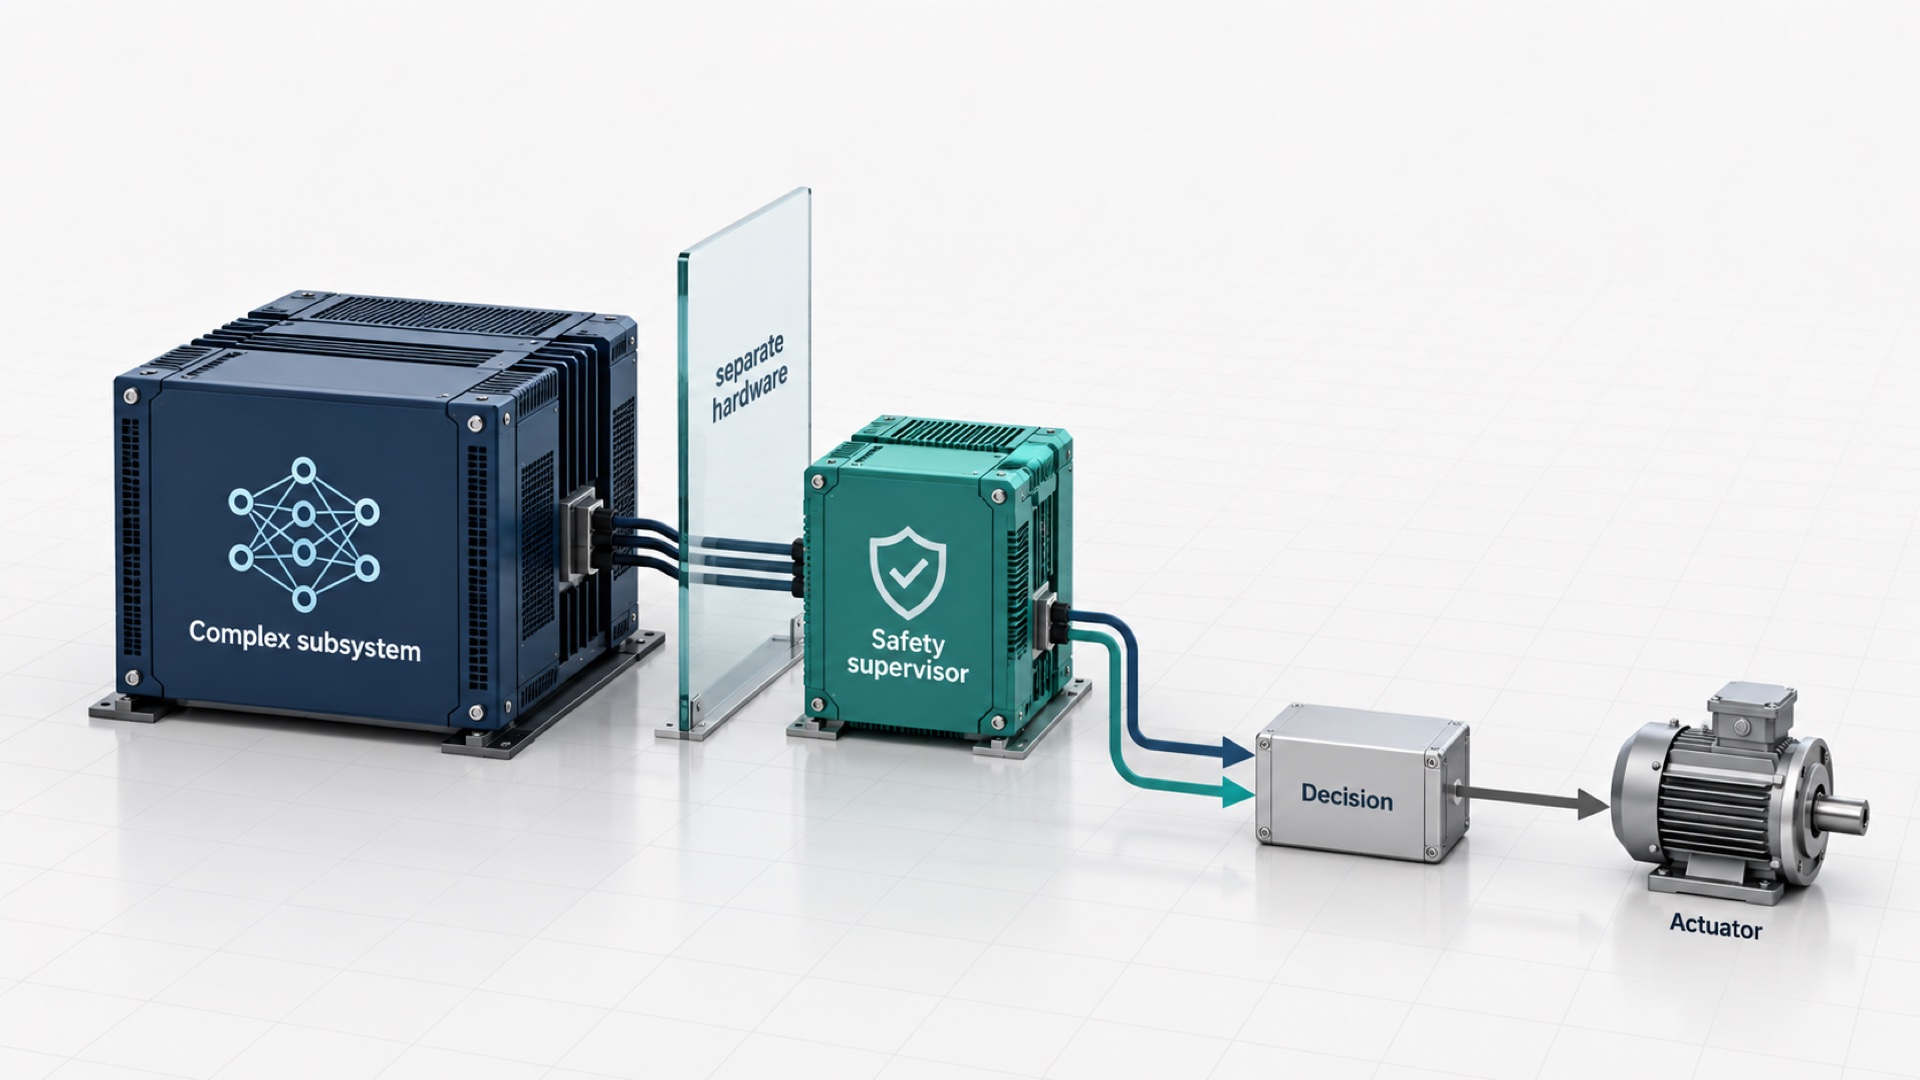
\includegraphics[width=.50\linewidth,height=.46\textheight,keepaspectratio,trim=0 80 0 80,clip]{images/V06.jpg}
\namedcap{4}{Kiến trúc Simplex: thành phần phức tạp (trái) chỉ đưa ra đề xuất; bộ giám sát an toàn trên phần cứng riêng (phải) quyết định tín hiệu cuối cùng gửi tới cơ cấu chấp hành.}
\end{minipage}
\note{Giám sát lấy cảm hứng từ Simplex; đầu ra mô phỏng, chưa chứng minh bộ điều khiển dự phòng.}
\end{frame}
\begin{frame}{2.2 Lập lịch thời gian thực trên Linux}
\small
\begin{columns}[T,onlytextwidth]
\begin{column}{.51\textwidth}
\begin{itemize}\setlength{\itemsep}{2pt}\setlength{\parsep}{0pt}\setlength{\parskip}{0pt}\setlength{\topsep}{0pt}
\item Bộ lập lịch (scheduler) là thành phần của hệ điều hành quyết định tác vụ nào được chạy trên CPU (Central Processing Unit) tại mỗi thời điểm.
\item \textbf{Hình 5 (trên, mặc định):} bộ lập lịch mặc định của Linux chia đều thời gian CPU. Tác vụ quan trọng (xanh) bị xen kẽ với tác vụ nền (xám) và phải chờ (khoảng cam), nên thời điểm hoàn thành dao động.
\item \textbf{Hình 5 (dưới, sau tinh chỉnh):} tác vụ quan trọng dùng chính sách SCHED\_FIFO (ưu tiên cố định) và được ghim riêng một nhân; tác vụ nền bị giới hạn bằng cgroups, nên tác vụ quan trọng chạy đều đặn.
\end{itemize}
\end{column}
\begin{column}{.47\textwidth}
\begin{minipage}{\linewidth}\centering\slideimg[.46\textheight]{\linewidth}{V11}{}\namedcap{5}{Lập lịch mặc định (trên) và sau tinh chỉnh (dưới); mỗi hàng là một nhân CPU, trục ngang là thời gian.}\end{minipage}
\end{column}
\end{columns}
\vspace{6pt}cgroups (control groups) là cơ chế giới hạn tài nguyên của nhóm tiến trình; ghim CPU chọn nhân được phép chạy.\par
\end{frame}
\begin{frame}{2.2 Lập lịch thời gian thực trên Linux (tiếp): PREEMPT\_RT}
\small
\begin{itemize}\setlength{\itemsep}{2pt}\setlength{\parsep}{0pt}\setlength{\parskip}{0pt}\setlength{\topsep}{0pt}\item \textbf{Kết quả công bố [6]:} Kernel PREEMPT\_RT giảm các đoạn kernel không thể ngắt: trên Raspberry Pi 5 dưới tải nặng, độ trễ xấu nhất giảm từ 1,8 ms xuống 0,22 ms [6].
\end{itemize}
\begin{itemize}\setlength{\itemsep}{2pt}\setlength{\parsep}{0pt}\setlength{\parskip}{0pt}\setlength{\topsep}{0pt}
\item Đây là kết quả công bố của tác giả [6], không phải số đo của nhóm; giá trị gốc là 1\,848 và 224 $\mu$s, SCHED\_FIFO ưu tiên 99.
\item PREEMPT\_RT được thử bằng kernel Real-time Ubuntu đóng gói sẵn (P3), không sửa hoặc tự biên dịch kernel.
\item Lịch đều ở Hình 5 chỉ minh họa tác động mong muốn; độ trễ đuôi và deadline vẫn phải đo dưới tải.
\end{itemize}
\note{V4 ghi [5] cho PREEMPT\_RT nhưng nguồn này là [6] trong danh mục hiện có; sửa số trích dẫn, giữ nguyên câu.}
\vspace{8pt}
Hình 5a so sánh hai giá trị xấu nhất đã công bố trong cùng nghiên cứu [6].
\par\vspace{5pt}
\begin{minipage}{\linewidth}\centering
\begin{tikzpicture}[x=4cm,y=.8cm,font=\small]
\draw[flow] (0,0)--(2.05,0) node[right] {ms};
\fill[navy] (0,.4) rectangle (1.848,.9);
\fill[teal] (0,1.3) rectangle (.224,1.8);
\node[left] at (0,.65) {Kernel mặc định};\node[right] at (1.848,.65) {1,848};
\node[left] at (0,1.55) {PREEMPT\_RT};\node[right] at (.224,1.55) {0,224};
\end{tikzpicture}
\namedcap{5a}{Kết quả công bố [6]: độ trễ xấu nhất giảm với PREEMPT\_RT; đây không phải số đo nền tảng của nhóm.}
\end{minipage}
\end{frame}
\begin{frame}{2.3 Tranh chấp tài nguyên trên vi xử lý đa nhân}
\small
\begin{itemize}\setlength{\itemsep}{2pt}\setlength{\parsep}{0pt}\setlength{\parskip}{0pt}\setlength{\topsep}{0pt}
\item Bốn nhân Cortex-A76 có L2 riêng nhưng dùng chung L3 2 MB và bộ nhớ LPDDR4X (Hình 6b) [7].
\item Ghim CPU quyết định tác vụ chạy ở nhân nào, nhưng không cô lập được băng thông bộ nhớ (Hình 6a) [4]; tác vụ AI trên CPU bị chậm đáng kể khi nhân khác tranh chấp bộ nhớ [5].
\end{itemize}
\begin{columns}[T,onlytextwidth]
\begin{column}{.48\textwidth}
\begin{minipage}{\linewidth}\centering\textbf{(a)}\par\slideimg[.46\textheight]{\linewidth}{V05}{}\namedcap{6a}{Minh họa tranh chấp: ba nhân đọc ghi bộ nhớ liên tục làm nghẽn đường truyền chung (vùng cam), tác vụ ở nhân 0 bị chậm theo.}\end{minipage}
\end{column}
\begin{column}{.48\textwidth}
\centering\textbf{(b)}\par
\begin{tikzpicture}[x=1cm,y=1cm,font=\footnotesize,
c/.style={draw=navy,fill=white,align=center,minimum width=1.85cm,minimum height=.70cm,inner sep=2pt}]
\foreach \i in {0,1,2,3}{
\node[c] (c\i) at (\i*2,0) {Cortex-A76\\L2 512 KB};
\draw[flow] (\i*2,-.37)--(\i*2,-.80);}
\node[c,fill=teal!12,minimum width=7.8cm] (l3) at (3,-1.15) {L3 2 MB (dùng chung)};
\node[c,minimum width=4cm] (mc) at (3,-2.15) {Bộ điều khiển bộ nhớ};
\draw[flow] (l3)--(mc);
\node[c] (dram) at (3,-3.45) {LPDDR4X};\draw[flow] (mc)--(dram);
\node[draw=navy,dashed,fit=(c0)(c3)(l3)(mc),inner sep=5pt] (soc) {};
\node[above=3pt of soc,font=\small\bfseries] {BCM2712};
\node[c] (rp) at (6,-3.45) {RP1 (I/O)};
\draw[flow] (soc.east)--++(.25,0)|-(rp.east);
\node[align=center,font=\footnotesize] at (6.1,-2.65) {PCIe 2.0 $\times$4};
\end{tikzpicture}
\namedcap{6b}{Sơ đồ khối BCM2712 trên Raspberry Pi 5: bốn nhân có L2 riêng nhưng dùng chung L3 và bộ nhớ.}
\end{column}
\end{columns}\note{L2/L3: bộ nhớ đệm cấp 2/3; LPDDR4X: Low-Power Double Data Rate 4X. PCIe: Peripheral Component Interconnect Express. RP1 nằm ngoài BCM2712; sơ đồ lược bỏ GPU và ngoại vi không liên quan. [7] xác nhận cache, LPDDR4X, kết nối RP1. V4 dùng [3,4], sửa thành [4,5] theo danh mục.}
\end{frame}
\setcounter{slidefigure}{6}
\begin{frame}{2.4 Tuổi thông tin (Age of Information)}
\small
\begin{columns}[T,onlytextwidth]
\begin{column}{.51\textwidth}
\begin{itemize}\setlength{\itemsep}{2pt}\setlength{\parsep}{0pt}\setlength{\parskip}{0pt}\setlength{\topsep}{0pt}
\item AoI (Age of Information), tuổi thông tin tại $t$: $\Delta(t)=t-u(t)$; $u(t)$ là lúc lấy mẫu của dữ liệu mới nhất đã nhận [2].
\item Hình 7: tuổi tăng giữa hai lần nhận, giảm khi có dữ liệu mới; vùng cam là thời gian vượt ngưỡng $\tau$.
\item Đo AoI trung bình, AoI đỉnh và tỉ lệ thời gian vượt ngưỡng.
\item Ưu tiên dữ liệu mới có thể giảm AoI so với FIFO (First-In, First-Out) [3]; không bảo đảm cận trên cứng.
\end{itemize}
\end{column}
\begin{column}{.47\textwidth}
\begin{minipage}{\linewidth}\centering\slideimg[.46\textheight]{\linewidth}{V20}{}\figcap{Tuổi thông tin tăng theo thời gian; các vùng cam biểu thị vi phạm ngưỡng độ mới.}\end{minipage}
\end{column}
\end{columns}
\end{frame}
\section{Thiết kế hệ thống}
\begin{frame}{3.1 Kiến trúc tổng thể}
\small
\begin{itemize}\setlength{\itemsep}{2pt}\setlength{\parsep}{0pt}\setlength{\parskip}{0pt}\setlength{\topsep}{0pt}
\item Hình 8 (trái): Linux tạo dữ liệu $\rightarrow$ suy luận $\rightarrow$ bridge (tiến trình cầu nối); tác vụ gây tải tranh chấp tài nguyên.
\item Hình 8 (phải): UART (Universal Asynchronous Receiver-Transmitter) $\rightarrow$ nhận khung $\rightarrow$ giám sát; bộ giám sát trực tiếp quyết định đầu ra an toàn, tác vụ báo trạng thái chạy riêng.
\item GPIO (General-Purpose Input/Output) là đường kiểm chứng đồng bộ, không truyền kết quả AI.
\end{itemize}
\begin{minipage}{\linewidth}\centering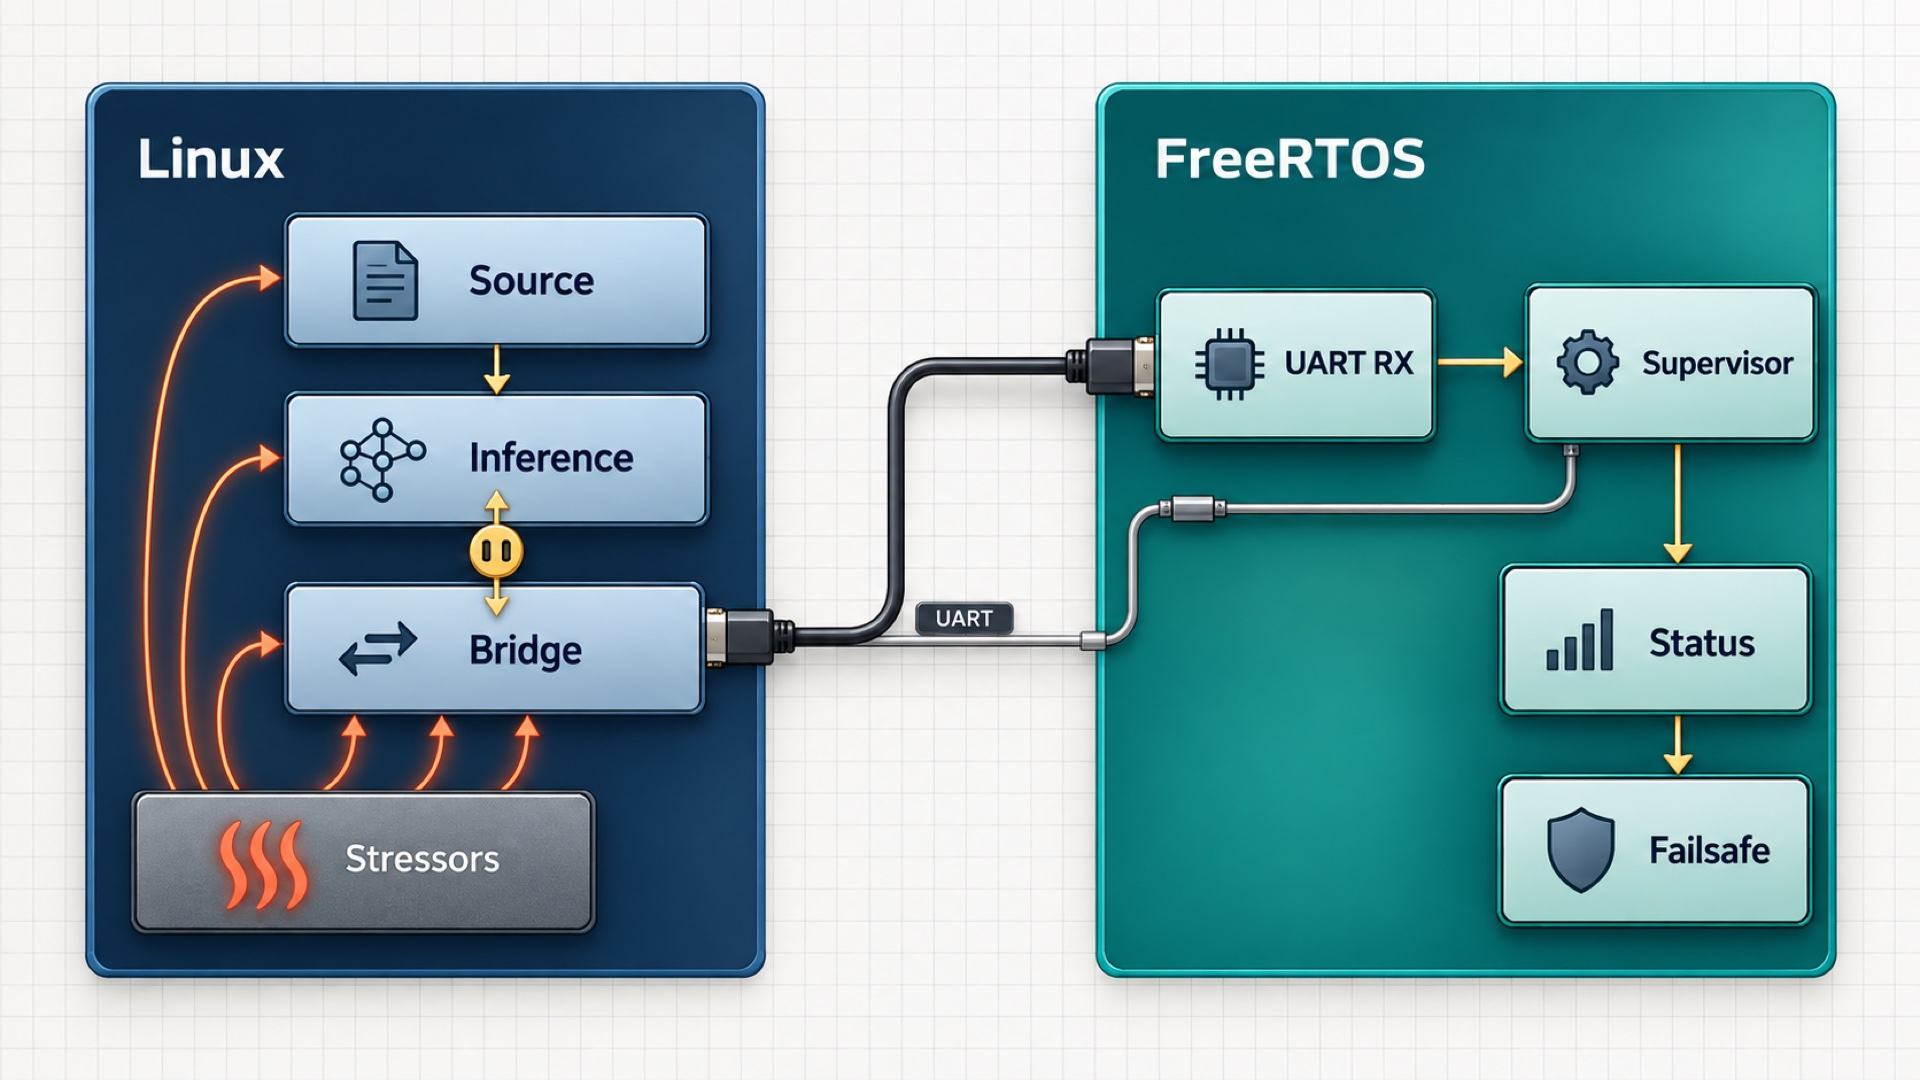
\includegraphics[width=\linewidth,height=.50\textheight,keepaspectratio,trim=0 35 0 35,clip]{images/V08.jpg}
\figcap{Hai miền Linux và FreeRTOS nối bằng UART; quyền quyết định đầu ra thuộc bộ giám sát độc lập.}\end{minipage}
\end{frame}
\begin{frame}{3.2 Phần cứng và đấu nối}
\relax
\small
\setlength{\parskip}{0pt}
\begin{columns}[T,onlytextwidth]
\begin{column}{.47\textwidth}
\small
\begin{minipage}{\linewidth}\centering\slideimg[.46\textheight]{\linewidth}{V22}{}\figcap{Đấu nối dự kiến: TX, RX, GND và GPIO đồng bộ; bảng bên phải xác định các đầu chân.}\end{minipage}
\end{column}
\begin{column}{.51\textwidth}
\small
Hình 9 minh họa bốn đường nối; cần xác nhận trên bo thật.\par\small\textbf{Đấu nối dự kiến}\par
\renewcommand{\arraystretch}{1.35}
\begin{tabular}{@{}L{.49\linewidth} L{.45\linewidth}@{}}
\toprule
\textbf{Raspberry Pi 5} & \textbf{STM32}\\\midrule
GPIO14 (TX, chân 8) & $\rightarrow$ PA10 (RX)\\
GPIO15 (RX, chân 10) & $\leftarrow$ PA9 (TX)\\
GND chân 6 & — GND\\
GPIO17 (chân 11) & $\rightarrow$ PA0 (TIM2\_CH1, đồng bộ)\\
\bottomrule
\end{tabular}\par
\end{column}
\end{columns}
\vspace{5pt}Raspberry Pi 5 4 GB, Ubuntu Server 24.04; Nucleo-F446RE (Cortex-M4F, 180 MHz), FreeRTOS.\par
GPIO (General-Purpose Input/Output) dùng cho tín hiệu đồng bộ.

\note{TX là Transmit, RX là Receive, GND là Ground. Xác nhận pin, UART controller, device node, baud và timer clock trên bo thật; vị trí jumper trong ảnh không phải sơ đồ chân đã xác minh.}
\end{frame}
\begin{frame}{3.3 Luồng dữ liệu của một kết quả}
\small
\begin{minipage}{\linewidth}\centering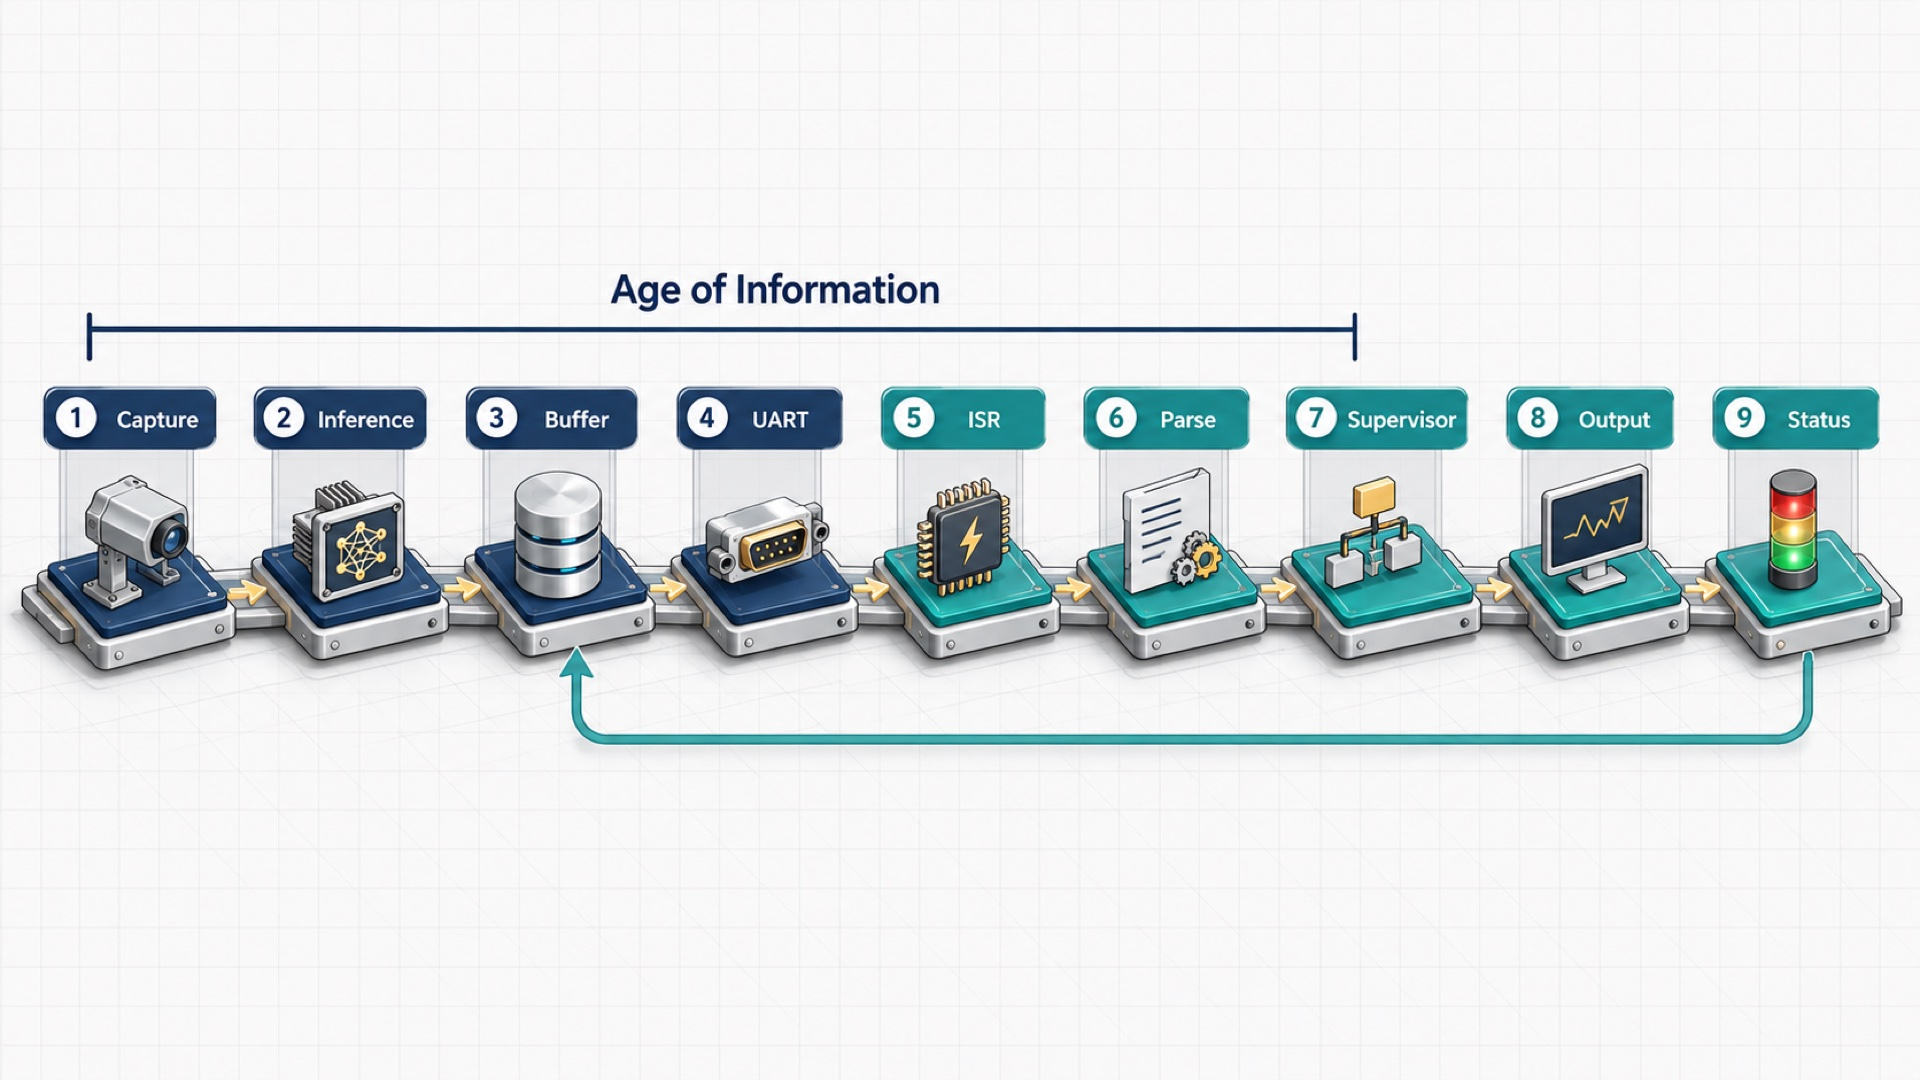
\includegraphics[width=\linewidth,keepaspectratio,trim=0 250 0 230,clip]{images/V10.jpg}
\figcap{Chín trạm của đường dữ liệu: theo dấu một mẫu đầu vào từ Linux đến quyết định và phản hồi STM32.}\end{minipage}
\begin{itemize}\setlength{\itemsep}{2pt}\setlength{\parsep}{0pt}\setlength{\parskip}{0pt}\setlength{\topsep}{0pt}
\item Hình 10, trạm 1–4: lấy mẫu và ghi $t_{input}$ $\rightarrow$ suy luận $\rightarrow$ bộ đệm $\rightarrow$ UART.
\item Trạm 5–8: ngắt nhận byte $\rightarrow$ phân tích khung $\rightarrow$ giám sát $\rightarrow$ đầu ra; trạm 9 báo trạng thái về Linux.
\item Ngoặc Age of Information nhấn mạnh tuổi từ lúc lấy mẫu; hình dừng ngoặc tại giám sát, còn phép đo đến đầu ra phải tính thêm trạm 8.
\end{itemize}
\note{MobileNetV2 trên ONNX Runtime CPU, FP32; chu kỳ dự kiến 100 ms. Khoảng công bố 20–50 ms không phải số đo nhóm và không dùng làm cận dưới tải.}
\end{frame}
\begin{frame}{3.4 Các cấu hình runtime}
\relax
\small
\setlength{\parskip}{0pt}
\begin{columns}[T,onlytextwidth]
\begin{column}{.47\textwidth}
\small
\begin{minipage}{\linewidth}\centering\slideimg[.46\textheight]{\linewidth}{V12}{}\figcap{P0 đến P1 là gói tinh chỉnh; P2 và P3 là hai nhánh độc lập từ P1.}\end{minipage}
\end{column}
\begin{column}{.51\textwidth}
\small
\small
\renewcommand{\arraystretch}{1.35}
\begin{tabular}{@{}L{.20\linewidth} L{.74\linewidth}@{}}
\toprule
\textbf{Cấu hình} & \textbf{Nội dung}\\\midrule
P0 & Linux mặc định\\
P1 & SCHED\_FIFO (ưu tiên 50), ghim CPU, giới hạn cgroups, khóa bộ nhớ (mlockall)\\
P2 & P1 + latest-value buffer\\
P3 & P1 trên kernel Real-time Ubuntu (PREEMPT\_RT)\\
\bottomrule
\end{tabular}\par
\end{column}
\end{columns}
\vspace{8pt}Hình 11: mũi tên P0$\rightarrow$P1 đánh giá gói tinh chỉnh; hai nhánh còn lại tách tác động bộ đệm và kernel: P0$\rightarrow$P1, P1$\rightarrow$P2, P1$\rightarrow$P3.
\note{Các cấu hình là dự kiến. P0–P1 đánh giá một gói tinh chỉnh; không tách riêng hiệu quả từng cơ chế trong gói. P2 và P3 là hai nhánh độc lập từ P1.}
\end{frame}
\begin{frame}{3.5 Latest-value buffer}
\small
\begin{columns}[T,onlytextwidth]
\begin{column}{.51\textwidth}
\begin{itemize}\setlength{\itemsep}{2pt}\setlength{\parsep}{0pt}\setlength{\parskip}{0pt}\setlength{\topsep}{0pt}
\item Latest-value buffer là bộ đệm một ô, giữ kết quả mới nhất chưa gửi.
\item Hình 12 (trên): FIFO giữ thứ tự đến; khi quá tải, các kết quả cũ phải chờ.
\item Hình 12 (dưới): kết quả mới thay kết quả cũ chưa gửi, hạn chế tồn đọng.
\item Không hủy suy luận hay khung đang truyền; kỳ vọng giảm AoI trung bình, không bảo đảm cận trên cứng.
\end{itemize}
\end{column}
\begin{column}{.47\textwidth}
\begin{minipage}{\linewidth}\centering\slideimg[.46\textheight]{\linewidth}{V14}{}\figcap{FIFO tích lũy dữ liệu cũ (trên); bộ đệm một ô thay dữ liệu chưa gửi bằng kết quả mới nhất (dưới).}\end{minipage}
\end{column}
\end{columns}
\end{frame}
\begin{frame}{3.6 Giao thức truyền UART}
\relax
\small
\setlength{\parskip}{0pt}
\centering\begin{tikzpicture}[
    f/.style={draw=navy,fill=white,minimum height=10mm,align=center,font=\small,inner sep=2pt},
    w/.style={font=\small,text=muted}]
    \node[f,fill=navy!10,minimum width=29mm] (sof) {SOF\\\texttt{A5 5A}};
    \node[f,minimum width=18mm,right=0pt of sof] (ver) {ver};
    \node[f,minimum width=18mm,right=0pt of ver] (typ) {type};
    \node[f,minimum width=18mm,right=0pt of typ] (seq) {seq};
    \node[f,minimum width=18mm,right=0pt of seq] (len) {len};
    \node[f,fill=teal!12,minimum width=61mm,right=0pt of len] (pay) {payload};
    \node[f,fill=navy!10,minimum width=29mm,right=0pt of pay] (crc) {CRC-16};
    \foreach \n/\b in {sof/2 B,ver/1 B,typ/1 B,seq/1 B,len/1 B,pay/$\le$64 B,crc/2 B}
      \node[w,below=2pt of \n] {\b};
    \draw[decorate,decoration={brace,amplitude=4pt},muted] (ver.north west)--node[above=5pt,w] {CRC bao phủ từ ver đến payload} (pay.north east);
  \end{tikzpicture}\figcap{Khung UART: dấu bắt đầu, header, payload và CRC; ngoặc chỉ các byte được kiểm tra CRC.}\begin{itemize}\setlength{\itemsep}{2pt}\setlength{\parsep}{0pt}\setlength{\parskip}{0pt}\setlength{\topsep}{0pt}
\item Hình 13: SOF (Start of Frame) là hai byte bắt đầu; header gồm phiên bản, loại, số thứ tự và độ dài; payload chứa dữ liệu tối đa 64 byte.
\item CRC (Cyclic Redundancy Check) phát hiện khung hỏng; “CRC bao phủ” nghĩa là tính trên các byte từ ver đến hết payload, không gồm SOF.
\item Bản tin: HEARTBEAT, INFERENCE, ECHO\_REQ/RESP và MCU\_STATUS (Microcontroller Unit: vi điều khiển).
\item Kiểm thử trên máy tính theo tài liệu dự án: phát hiện toàn bộ lỗi một bit; khôi phục 99,99\% khung dưới nhiễu ngẫu nhiên. Chưa kiểm chứng UART thật.
\end{itemize}
\note{SOF (Start of Frame) là hai byte bắt đầu khung. MCU (Microcontroller Unit) là vi điều khiển. Kết quả kiểm thử phần mềm được brief ghi nhận; chưa đo độ tin cậy đường UART thật.}
\end{frame}
\begin{frame}{3.7 Bộ giám sát trên STM32}
\relax
\small
\setlength{\parskip}{0pt}
\begin{columns}[T,onlytextwidth]
\begin{column}{.57\textwidth}
\small
\raggedright\begin{tikzpicture}[
        st/.style={draw=navy,fill=white,rounded corners=3pt,minimum width=20mm,minimum height=10mm,font=\small\bfseries,thick},
        lb/.style={lbl,font=\small,inner sep=2pt}]
        \node[st] (init) at (0,0) {INIT};
        \node[st,fill=teal!15] (fresh) at (3.1,0) {FRESH};
        \node[st,fill=navy!10] (hold) at (3.1,-2.7) {HOLD};
        \node[st,draw=fault,fill=fault!15,text=fault] (fs) at (6.2,-1.35) {FAILSAFE};
        \node[font=\small,text=fault,below=1pt of fs] {Giữ chốt};
        \draw[flow] (init)--node[lb,above=10pt] {Dữ liệu hợp lệ} (fresh);
        \draw[flow] (fresh.250)--node[lb,left] {Quá cũ} (hold.110);
        \draw[flow] (hold.70)--node[lb,right] {Mới lại} (fresh.290);
        \draw[faultflow] (fresh.east)--node[lb,above=2pt,sloped] {Mất heartbeat} (fs.north west);
        \draw[faultflow] (hold.east)--node[lb,below=2pt,sloped] {Mất heartbeat} (fs.south west);
        \draw[flow,dashed] (fs.north)--(6.2,1.25)--node[lb,above] {Khởi động lại rõ ràng} (0,1.25)--(init.north);
      \end{tikzpicture}\figcap{Bộ giám sát chuyển FRESH sang HOLD khi dữ liệu cũ; mất heartbeat dẫn đến FAILSAFE giữ chốt.}\end{column}
\begin{column}{.41\textwidth}
\small
\begin{itemize}\setlength{\itemsep}{2pt}\setlength{\parsep}{0pt}\setlength{\parskip}{0pt}\setlength{\topsep}{0pt}
\item Hình 14 dùng hai bộ định thời độc lập: heartbeat (bridge còn hoạt động) và độ mới của kết quả.
\item INIT $\rightarrow$ FRESH khi có dữ liệu hợp lệ; dữ liệu cũ: FRESH $\rightarrow$ HOLD; mất heartbeat: chuyển thẳng FAILSAFE.
\item HOLD $\rightarrow$ FRESH khi có dữ liệu mới. FAILSAFE được chốt, chỉ thoát khi có lệnh khởi động lại rõ ràng.
\item Khung trùng lặp hoặc sai CRC không làm mới bộ định thời.
\end{itemize}
\end{column}
\end{columns}

\note{Đây là thiết kế cần triển khai. INIT chưa áp dụng đề xuất Linux; HOLD dùng trạng thái dự phòng. Skeleton hiện mới có một bộ định thời; đồng bộ và sai số đồng hồ phải được kiểm chứng.}
\end{frame}
\begin{frame}{3.8 Vì sao cần hai bộ định thời}
\small
\begin{itemize}\setlength{\itemsep}{2pt}\setlength{\parsep}{0pt}\setlength{\parskip}{0pt}\setlength{\topsep}{0pt}
\item Hình 15, hàng trên: heartbeat vẫn có xung đều, cho biết bridge còn hoạt động.
\item Hàng dưới: tuổi kết quả không giảm khi suy luận ngừng cập nhật; đường răng cưa vượt ngưỡng và bộ giám sát phát hiện dữ liệu cũ.
\item Vì vậy cần kiểm tra cả hoạt động của bridge và độ mới; supervisor có ưu tiên ứng dụng cao nhất, chu kỳ dự kiến 1 kHz.
\end{itemize}
\begin{minipage}{\linewidth}\centering\slideimg[.55\textheight]{\linewidth}{V17}{}\figcap{Heartbeat vẫn đều nhưng tuổi kết quả vượt ngưỡng; một bộ định thời hoạt động không phát hiện được dữ liệu cũ.}\end{minipage}\note{Tuổi giảm về trễ giao nhận, không về 0 như hình minh họa. Chu kỳ là thiết kế, chưa đo.}
\end{frame}
\begin{frame}{3.9 Đồng bộ đồng hồ giữa hai miền}
\relax
\small
\setlength{\parskip}{0pt}
\begin{columns}[T,onlytextwidth]
\begin{column}{.51\textwidth}
\small
\centering\begin{tikzpicture}[font=\small]
        \draw[navy,thick] (0,0) node[above,align=center] {\textbf{Linux}\\Đồng hồ monotonic}--(0,-3.8);
        \draw[teal,thick] (3.8,0) node[above,align=center] {\textbf{STM32}\\Bộ định thời}--(3.8,-3.8);
        \draw[flow] (0,-.5) node[left] {$T_1$}--node[lbl,above,sloped] {ECHO\_REQ} (3.8,-1.4) node[right] {$T_2$};
        \draw[flow,teal] (3.8,-2.1) node[right] {$T_3$}--node[lbl,above,sloped] {ECHO\_RESP} (0,-3.1) node[left] {$T_4$};
        \foreach \y in {-.5,-3.1} \fill[navy] (0,\y) circle (1.5pt);
        \foreach \y in {-1.4,-2.1} \fill[teal] (3.8,\y) circle (1.5pt);
      \end{tikzpicture}\figcap{T1–T4 là các mốc gửi/nhận qua UART; trao đổi hai chiều ước lượng độ lệch hai đồng hồ.}\end{column}
\begin{column}{.47\textwidth}
\small
Hình 16: $T_1$ Linux gửi, $T_2$ STM32 nhận; $T_3$ STM32 trả lời, $T_4$ Linux nhận.\par
$\theta$: độ lệch đồng hồ; $\delta$: trễ khứ hồi [8].
\[\theta=\frac{(T_2-T_1)+(T_3-T_4)}{2}\]
\[\delta=(T_4-T_1)-(T_3-T_2)\]
Giả thiết trễ hai chiều đối xứng.\par
\begin{itemize}\setlength{\itemsep}{2pt}\setlength{\parsep}{0pt}\setlength{\parskip}{0pt}\setlength{\topsep}{0pt}
\item Đồng hồ Linux CLOCK\_MONOTONIC\_RAW (ns) và bộ định thời STM32 ($\mu$s).
\item Cạnh GPIO trên PA0 dùng làm chuẩn kiểm chứng độc lập.
\end{itemize}
\end{column}
\end{columns}

\note{Quy đổi cùng đơn vị trước khi tính offset và trễ khứ hồi; ước lượng drift qua nhiều trao đổi. Công thức theo RFC 4330, mục 5. GPIO Linux userspace không cung cấp thời điểm cạnh vật lý chính xác; cần timer input capture và kiểm chứng ngoài Linux.}
\end{frame}
\section{Phương pháp đánh giá}
\begin{frame}{4.1 Chỉ số đánh giá}
\relax
\small
\setlength{\parskip}{0pt}
\renewcommand{\arraystretch}{1.35}
\begin{tabular}{@{}L{.20\textwidth} L{.74\textwidth}@{}}
\toprule
\textbf{Nhóm} & \textbf{Chỉ số}\\\midrule
Độ trễ & P50, P99, giá trị lớn nhất (từ lúc lấy mẫu đến lúc STM32 nhận)\\
Độ mới & AoI trung bình, AoI đỉnh, tỉ lệ vượt ngưỡng $V(\tau)$\\
Phản ứng lỗi & Thời gian phát hiện, thời gian kích hoạt, tổng thời gian đến đầu ra an toàn\\
Độ tin cậy & Số deadline bị lỡ trên tổng số chu kỳ\\
\bottomrule
\end{tabular}\par

\note{P50 và P99 là phân vị 50 và 99 phần trăm. Tính tỉ lệ lỡ deadline trên toàn bộ chu kỳ đầu vào, kể cả kết quả bị thay thế. AoI gồm khoảng chưa có cập nhật mới.}
\vspace{12pt}
\begin{itemize}\setlength{\itemsep}{4pt}
\item P50/P99 là phân vị 50/99\%: phân biệt hành vi thường gặp và các mẫu chậm ở đuôi phân bố.
\item $V(\tau)=\frac{\text{thời gian AoI vượt }\tau}{\text{tổng thời gian quan sát}}$: đo khoảng hệ thống dùng dữ liệu quá cũ.
\item Deadline là hạn hoàn thành; mẫu bị thay trong bộ đệm vẫn được tính trong tổng số chu kỳ đầu vào.
\item Giá trị lớn nhất quan sát là kết quả của lần đo, chưa chứng minh cận trên cho mọi trường hợp.
\end{itemize}
\end{frame}
\begin{frame}{4.2 Các thí nghiệm}
\relax
\small
\setlength{\parskip}{0pt}
\renewcommand{\arraystretch}{1.35}
\begin{tabular}{@{}L{.18\textwidth} L{.43\textwidth} L{.32\textwidth}@{}}
\toprule
\textbf{Thí nghiệm} & \textbf{So sánh} & \textbf{Mục đích}\\\midrule
E1 & P0 khi rảnh và dưới tải CPU, bộ nhớ, cache, I/O (Input/Output) & Đo ảnh hưởng của tranh chấp\\
E2 & P0 với P1; P1 với P3 & Hiệu quả của tinh chỉnh và kernel\\
E3 & P1 với P2 khi tải tăng & Hiệu quả của latest-value buffer\\
E4 & Dừng bridge, treo tiến trình, chiếm CPU & Độ trễ chuyển sang failsafe\\
\bottomrule
\end{tabular}\par
\vspace{12pt}Mọi lần chạy ghi nhiệt độ, tần số CPU; loại bỏ lần chạy bị giảm xung (throttling).
\note{Lưu cả lượt bị loại và lý do; không bỏ mẫu trễ trong lượt hợp lệ. Giữ workload, chu kỳ, tải, governor và làm nóng tương đương; lặp độc lập và xáo thứ tự chạy.}
\end{frame}
\begin{frame}{4.3 Đo phản ứng khi có lỗi}
\small
\begin{columns}[T,onlytextwidth]
\begin{column}{.51\textwidth}
\begin{itemize}\setlength{\itemsep}{2pt}\setlength{\parsep}{0pt}\setlength{\parskip}{0pt}\setlength{\topsep}{0pt}
\item Hình 17, hàng heartbeat: xung dừng tại Fault, mốc lỗi $t_f$; hàng State đổi tại quyết định $t_d$; hàng Output đổi tại đầu ra an toàn $t_s$.
\item Reaction time $=t_s-t_f$; tách thời gian phát hiện $t_d-t_f$ và kích hoạt $t_s-t_d$.
\item Logic analyzer (máy phân tích logic) ghi ba mốc trên cùng đồng hồ ngoài Linux; log Linux không đo được lúc Linux treo.
\item Ngân sách dự kiến: timeout + chu kỳ giám sát + trễ điều phối + thực thi + trễ đầu ra.
\end{itemize}
\end{column}
\begin{column}{.47\textwidth}
\begin{minipage}{\linewidth}\centering\slideimg[.46\textheight]{\linewidth}{V23}{}\figcap{Heartbeat dừng, trạng thái đổi, đầu ra an toàn bật: ba mốc được đo bằng đồng hồ ngoài Linux.}\end{minipage}
\end{column}
\end{columns}\note{Giá trị lớn nhất quan sát không chứng minh cận trên mọi trường hợp.}
\end{frame}
\begin{frame}{4.4 Giả thuyết}
\relax
\small
\setlength{\parskip}{0pt}
\renewcommand{\arraystretch}{1.35}
\begin{tabular}{@{}L{.13\textwidth} L{.81\textwidth}@{}}
\toprule
\textbf{Giả thuyết} & \textbf{Nội dung}\\\midrule
H1 & Tranh chấp làm tăng P99 nhiều hơn hẳn P50.\\
H2 & Tinh chỉnh khôi phục độ trễ đuôi do tranh chấp CPU nhưng không khôi phục được tranh chấp bộ nhớ.\\
H3 & Latest-value buffer giảm AoI trung bình và thời gian vượt ngưỡng.\\
H4 & Thời gian chuyển sang failsafe luôn nằm trong ngân sách với mọi loại lỗi.\\
\bottomrule
\end{tabular}\par

\note{H1–H4 là giả thuyết, chưa phải kết quả. H4 được kiểm tra với các loại lỗi E4 và ngân sách đầy đủ; thử nghiệm hữu hạn không chứng minh bảo đảm cho mọi lỗi có thể xảy ra.}
\vspace{12pt}
\begin{itemize}\setlength{\itemsep}{4pt}
\item H1 được kiểm tra bằng E1; H2 bằng E2; H3 bằng E3; H4 bằng E4.
\item Đây là dự đoán cần kiểm định, chưa phải kết quả. H4 chỉ được đánh giá trong tập lỗi và điều kiện đã thử.
\item Báo cáo cả giả thuyết bị bác bỏ; giữ mẫu trễ trong lượt hợp lệ để tránh làm đẹp kết quả.
\end{itemize}
\end{frame}
\section{Tiến độ và kế hoạch}
\begin{frame}{5.1 Kết quả đã đạt được}
\relax
\small
\setlength{\parskip}{0pt}
\renewcommand{\arraystretch}{1.35}
\begin{tabular}{@{}L{.52\textwidth} L{.42\textwidth}@{}}
\toprule
\textbf{Hạng mục} & \textbf{Trạng thái}\\\midrule
Thiết kế và khảo sát tài liệu & Hoàn thành\\
Thư viện giao thức + kiểm thử trên máy tính & Hoàn thành\\
Máy trạng thái giám sát (bản đầu, một bộ định thời) & Có kiểm thử, cần nâng cấp hai bộ định thời\\
CI (Continuous Integration) và script cài đặt Raspberry Pi & Hoàn thành, chưa chạy trên phần cứng\\
Firmware, bridge, thí nghiệm & Chưa thực hiện\\
\bottomrule
\end{tabular}\par

\note{Tiến độ theo tài liệu dự án ngày 06/10/2026; không chạy lại kiểm thử giao thức trong lần sửa slide. Cross-compile và CI không thay cho kiểm thử Raspberry Pi hoặc STM32 thật.}
\vspace{12pt}
\begin{itemize}\setlength{\itemsep}{4pt}
\item Các kết quả hiện tại xác nhận thiết kế và phần mềm trên máy tính; chưa có số đo Raspberry Pi 5 hoặc STM32.
\item Điểm chuyển tiếp: nâng cấp bộ giám sát hai bộ định thời, giữ chốt FAILSAFE và kiểm chứng bằng đường UART thật.
\end{itemize}
\end{frame}
\begin{frame}{5.2 Kế hoạch tiếp theo}
\relax
\small
\setlength{\parskip}{0pt}
\begin{enumerate}
\item Lắp đặt và kiểm tra phần cứng.
\item Bộ giám sát hai bộ định thời và đồng bộ đồng hồ.
\item Bridge trên Linux và firmware FreeRTOS.
\item Kiểm tra đường truyền và đồng bộ bằng GPIO.
\item Thực hiện E1–E4.
\item Viết báo cáo.
\end{enumerate}
\vspace{8pt}
Hình 17a nhóm sáu bước thành ba giai đoạn có đầu ra kiểm chứng được.
\par\vspace{6pt}
\begin{minipage}{\linewidth}\centering
\begin{tikzpicture}[node distance=10mm,box/.append style={minimum width=45mm,minimum height=15mm}]
\node[box] (a) {Bước 1–3\\Lắp ráp và triển khai};
\node[box,right=of a] (b) {Bước 4\\Kiểm chứng đường đo};
\node[box,right=of b] (c) {Bước 5–6\\Thí nghiệm và báo cáo};
\draw[flow] (a)--(b);\draw[flow] (b)--(c);
\end{tikzpicture}
\namedcap{17a}{Trình tự thực hiện: chỉ đo E1–E4 sau khi đường truyền và đồng bộ được kiểm chứng.}
\end{minipage}
\end{frame}
\section{Kết luận}
\begin{frame}{6.1 Kết luận}
\small
\begin{columns}[T,onlytextwidth]\begin{column}{.58\textwidth}
\begin{itemize}\setlength{\itemsep}{2pt}\setlength{\parsep}{0pt}\setlength{\parskip}{0pt}\setlength{\topsep}{0pt}
\item AI trên thiết bị biên ngày càng điều khiển trực tiếp hệ thống vật lý, nên kết quả phải vừa đúng vừa kịp thời; Linux đơn thuần tối ưu thông lượng và không bảo đảm điều này.
\item Đồ án đề xuất một nền tảng không đồng nhất Linux + FreeRTOS theo kiến trúc Simplex, với latest-value buffer, bộ giám sát hai bộ định thời và đồng bộ đồng hồ, chỉ dùng cơ chế sẵn có của hệ điều hành.
\item Ý nghĩa: hướng kiến trúc này phù hợp xu hướng SoC tích hợp nhân ứng dụng và nhân thời gian thực; các phép đo sẽ chỉ ra cơ chế nào thực sự cần thiết và chi phí của chúng, làm cơ sở thiết kế cho robot, drone và máy công nghiệp dùng AI.
\item Hiện trạng: đã hoàn thành thiết kế, thư viện giao thức và kế hoạch thí nghiệm; bước tiếp theo là triển khai trên phần cứng để trả lời RQ1–RQ3 bằng số liệu đo.
\end{itemize}
\end{column}\begin{column}{.40\textwidth}
Hình 18 nhắc lại hai miền: Linux đề xuất, STM32 quyết định đầu ra.
\begin{minipage}{\linewidth}\centering\slideimg[.42\textheight]{\linewidth}{V08}{}\figcap{Kiến trúc đề xuất.}\end{minipage}\par
\vspace{8pt}\raggedright
Phép đo dùng đồng hồ ngoài Linux để quan sát cả lúc Linux ngừng phản hồi.\par
\vspace{5pt}Nền tảng chi phí thấp, có thể tái lập; phù hợp giảng dạy cơ chế hệ điều hành và đo hệ thống Edge-AI.
\end{column}\end{columns}
\end{frame}
\begingroup
\linespread{0.88}
\begin{frame}{Tài liệu tham khảo (1/3)}
\relax
\small
\setlength{\parskip}{0pt}
\begin{thebibliography}{9}
    \setlength{\itemsep}{2pt}
    \bibitem{bak2009} Stanley Bak, Deepti K. Chivukula, Olugbemiga Adekunle,
      Mu Sun, Marco Caccamo, Lui Sha.\par
      The System-Level Simplex Architecture for Improved Real-Time Embedded System Safety.\par
      \emph{IEEE RTAS},
      2009, pp.~99--107.
      \href{https://dblp.org/rec/conf/rtas/BakCASCS09}{[DBLP]}
    \bibitem{kaul2012infocom} Sanjit Krishnan Kaul, Roy D. Yates, Marco Gruteser.\par
      Real-time status: How often should one update?\par
      \emph{IEEE INFOCOM}, 2012, pp.~2731--2735.
      \href{https://dblp.org/rec/conf/infocom/KaulYG12.html}{[DBLP]}
    \bibitem{kaul2012queues} Sanjit Krishnan Kaul, Roy D. Yates, Marco Gruteser.\par
      Status updates through queues.\par
      \emph{CISS}, 2012, pp.~1--6.
      \href{https://dblp.org/rec/conf/ciss/KaulYG12}{[DBLP]}
  \end{thebibliography}
\end{frame}
\endgroup
\begingroup
\linespread{0.88}
\begin{frame}{Tài liệu tham khảo (2/3)}
\relax
\small
\setlength{\parskip}{0pt}
\begin{thebibliography}{9}
    \setcounter{enumiv}{3}
    \setlength{\itemsep}{2pt}
    \bibitem{yun2013memguard} Heechul Yun, Gang Yao, Rodolfo Pellizzoni, Marco Caccamo, Lui Sha.\par
      MemGuard: Memory bandwidth reservation system for efficient performance isolation
      in multi-core platforms.\par
      \emph{IEEE RTAS},
      2013, pp.~55--64.
      \href{https://dblp.org/rec/conf/rtas/YunYPCS13.html}{[DBLP]}
    \bibitem{bechtel2018deeppicar} Michael Garrett Bechtel, Elise McEllhiney, Minje Kim, Heechul Yun.\par
      DeepPicar: A Low-Cost Deep Neural Network-Based Autonomous Car.\par
      \emph{IEEE RTCSA}, 2018, pp.~11--21.
      \href{https://dblp.org/rec/conf/rtcsa/BechtelMKY18.html}{[DBLP]}
    \bibitem{arxiv2604} Luiz Giacomossi, Håkan Forsberg, Ivan Tomasic, Baran Çürüklü,
      Tommaso Cucinotta.\par
      Scheduling Analysis of UAV Flight Control Workloads on PREEMPT\_RT Linux
      Using a Raspberry Pi~5.\par
      \emph{arXiv:2604.19275}, 2026 (v2).
      \href{https://arxiv.org/abs/2604.19275}{[arXiv]}
  \end{thebibliography}
\end{frame}
\endgroup
\begin{frame}{Tài liệu tham khảo (3/3)}
\small
\begin{thebibliography}{9}\setcounter{enumiv}{6}
\bibitem{bcm2712} Raspberry Pi Ltd.\par
BCM2712: cấu trúc bộ xử lý và hệ thống bộ nhớ.\par
\href{https://www.raspberrypi.com/documentation/computers/processors.html\#bcm2712}{Raspberry Pi Documentation};
\href{https://datasheets.raspberrypi.com/rp1/rp1-peripherals.pdf}{RP1 Peripherals: PCIe 2.0 $\times$4}. Truy cập 07/10/2026.
\bibitem{rfc4330} D. Mills.\par
Simple Network Time Protocol (SNTP), RFC 4330, mục 5, 2006.\par
\href{https://www.rfc-editor.org/rfc/rfc4330\#section-5}{Trao đổi bốn mốc thời gian và ước lượng độ lệch.}
\end{thebibliography}
\end{frame}
\begin{frame}[c]
\relax
\small
\setlength{\parskip}{0pt}
\centering{\LARGE\bfseries\color{navy}Cảm ơn thầy và các bạn đã lắng nghe!\par}
\end{frame}
\end{document}
